\documentclass[aspectratio=169]{beamer}

% beamer config
\usetheme{Berkeley}
% \AtBeginSection{\frame{\sectionpage}}

% package imports
\usepackage{graphicx}
\graphicspath{{./figs/}}

% Macros
\newcommand{\todo}[1]{\textcolor{red}{\textbf{[#1]}}}

\title[PhotoHunter]{PhotoHunter: A Citizen-Scientist Game with User-in-the-loop 
  Data Confirmation for Collecting Computer Vision Datasets of 
  Geo-tagged Imagery through Crowd-Sourcing Data Collection; 
  Abstracting Research using an Interactive, Game-based Mobile 
  Application for Large Dataset Creation}

\author[]{Connor Greenwell \and Ryan Baltenberger 
  \and J.\ David Smith \and Aaron Bradshaw}

\institute{QuesoTech.com}

\begin{document}

\maketitle

\section{Computer Vision}

\begin{frame}{Computer Vision}
  \begin{itemize}

    \item Artificial Intelligence - the goal of creating intelligence for
          machines/software

    \item Computer Vision - teaching computers to understand the natural world
          through images

    \item Data to train or test on is integral to success

    \item Collecting and labeling data is time consuming

  \end{itemize}
\end{frame}

\section{Citizen-Science}

\begin{frame}{Citizen-Science}
  \begin{itemize}
    
    \item Citizen-Science - form of crowd-sourcing where participants
          collect/analyze data

    \item Typically performed tasks are simple (\textit{e.g.} take a photo,
          measure temperature, translate text, etc.)

    \item Humans can perform simple tasks easily and in large quantities,
          often with little time or effort

    \item Collecting large amounts of data is intractable for a single 
          researcher

  \end{itemize}
\end{frame}

\section{Why a game?}

\begin{frame}{Why a Game?}
  \begin{itemize}
    
    \item Contributions to citizen-science style datasets drop off after
          the initial interest wears off
  
    \item Using ``gamification'' can mitigate this decline
  
    \item Our goal - abstract out the data collection, tell users they
          are competing in a global scavenger hunt

    \item Users will stay engaged/contributing to earn more points

    \item PhotoHunter will assign points for collecting and reviewing data

    \item Leader-boards will encourage competition between users

  \end{itemize}
\end{frame}

\section{Overview}

\begin{frame}{Overview}
  \todo{Flowchart}
\end{frame}

\section{Backend}

\begin{frame}{Backend}
  Research groups may be created on request. 

  Research groups will have an interface where they may request
  datasets. From this interface groups may define GPS bounding boxes,
  time frames, and other metadata they are interested in for a given
  dataset.
\end{frame}

\begin{frame}{Researchers Interface}
  \centering
  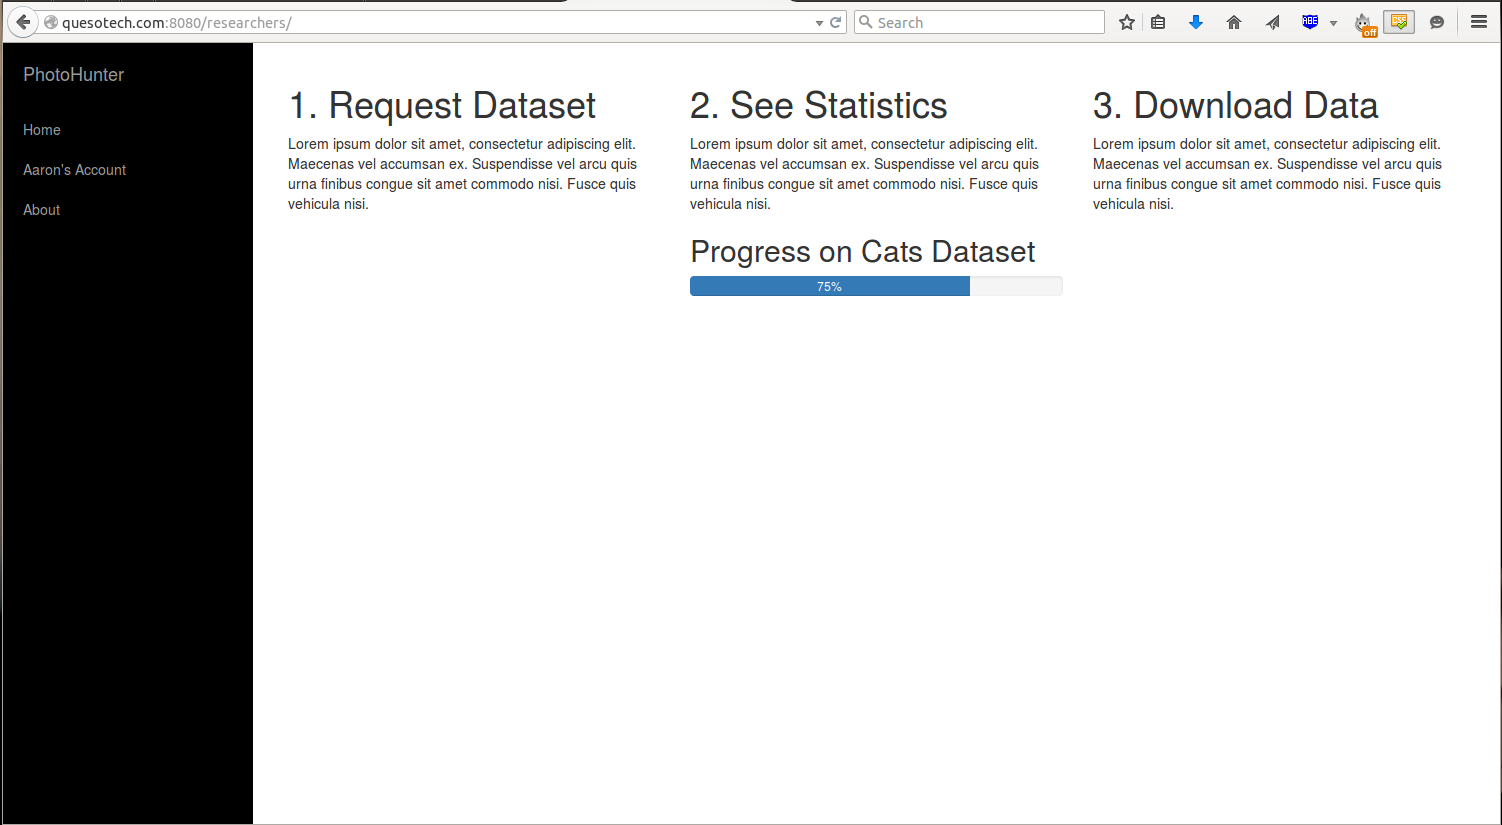
\includegraphics[width=\textwidth,height=\textheight,keepaspectratio]{researchers}
\end{frame}

\begin{frame}
  \todo{mockups}
\end{frame}

\begin{frame}{ER Diagram}
  \centering
  \includegraphics[width=\textwidth,height=\textheight,keepaspectratio]{er}
\end{frame}

\section{PhotoHunter}

\begin{frame}{PhotoHunter}
  From the mobile app, users will be presented with a list of
  datapoints
  to go collect in their area, and a time limit in which each must be
  completed. As each task is completed, they will gain points,
  prompting
  them to continue.

  Data collection will only occur within the mobile app so that we may
  take advantage of built in sensors (time, GPS, heading, etc.).
\end{frame}

\begin{frame}{PhotoHunter}
  \begin{columns}[c]
    \begin{column}{0.5\columnwidth}
      \centering
      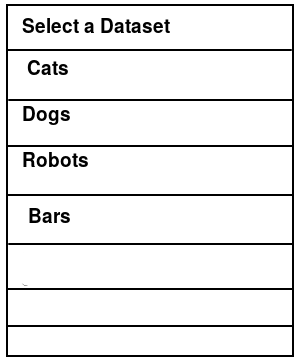
\includegraphics[width=\textwidth,height=\textheight,keepaspectratio]{ss_photohunter_dataset}
    \end{column}
    \begin{column}{0.5\columnwidth}
      \centering
      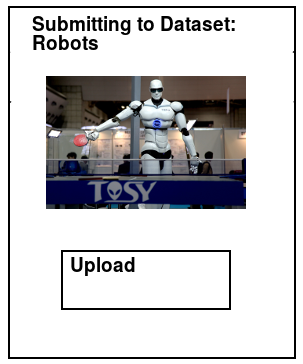
\includegraphics[width=\textwidth,height=\textheight,keepaspectratio]{ss_photohunter_upload}
    \end{column}
  \end{columns}
\end{frame}

\section{QuickPic}

\begin{frame}{QuickPic}
  For numerous reasons, users may unknowingly (or knowingly) submit
  incorrect data. For example, a dataset that is seeking pictures of
  fire hydrants may accidentally receive images of dogs, or trees. In
  this case we will employ users to filter submissions. When an image
  is
  submitted, it will be posted for confirmation by other users. The
  interface for this will display the image in question, the
  requirements, and a simple ``thumbs-up'' and ``thumbs-down'' option.
  Each image will be presented for confirmation to numerous users
  until
  we can be reasonably certain that the datapoint should be trusted.
\end{frame}

\begin{frame}{QuickPic}
  \begin{columns}[c]
    \begin{column}{0.5\columnwidth}
      \centering
      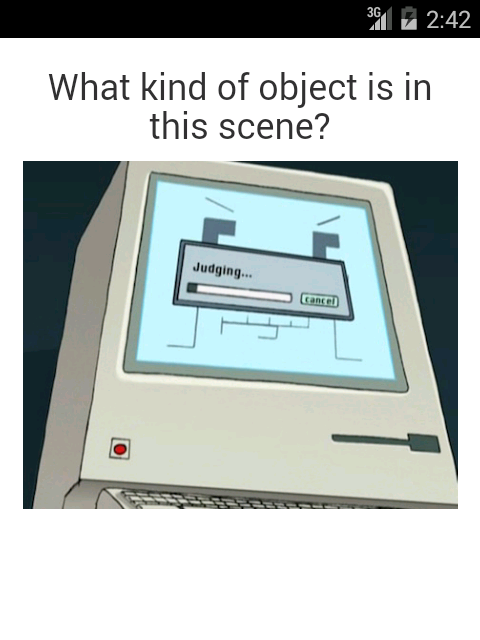
\includegraphics[width=\textwidth,height=\textheight,keepaspectratio]{ss_quickpic_image}
    \end{column}
    \begin{column}{0.5\columnwidth}
      \centering
      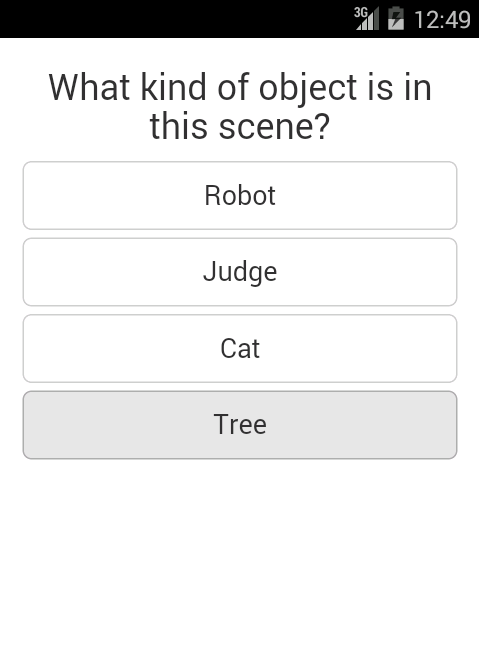
\includegraphics[width=\textwidth,height=\textheight,keepaspectratio]{ss_quickpic_options}
    \end{column}
  \end{columns}
\end{frame}

\frame{\centering Thanks!}

\end{document}
